%\documentclass{article}
%\usepackage{graphicx,subfigure}
%\begin{document}

\begin{figure}[!h]
  \centering
  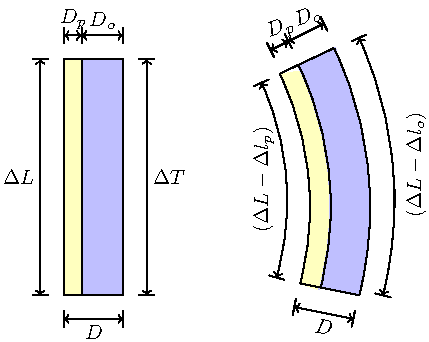
\includegraphics[width=0.9\textwidth]{fibre.pdf}
  \caption{Short lengths of fibre showing the initially straight and curved positions due to differential shortening of the para and ortho cortex segments, which are coloured yellow and blue respectively}
  \label{fig:fibre}
\end{figure}

%\end{document}

